%Class
\documentclass[12pt]{article}

%Package
\usepackage{multicol} 
\usepackage{graphicx}
\graphicspath{{/Users/DJYoon/Desktop/LaTex/}}
\DeclareGraphicsExtensions{.pdf,.png,.jpg,.jpeg}
\usepackage{listings}
\usepackage{color}
\definecolor{dkgreen}{rgb}{0,0.6,0}
\definecolor{gray}{rgb}{0.5,0.5,0.5}
\definecolor{mauve}{rgb}{0.58,0,0.82}



%Page
\usepackage{geometry}
\geometry{legalpaper, portrait}

%Header and Footer
\usepackage{fancyhdr}
\pagestyle{fancy}

%Title
\begin{document}
\begin{titlepage}
\begin{center}
\line(2,0){300}\\	
\huge{\bfseries Head Scope} \\
\textsc{\large Application for Head Mounted Display}\\[2\baselineskip]
\end{center} 

%HYU Image
\center

\includegraphics{TeamName}
\\ [9\baselineskip]


%Taehun(Top Left) 

\begin{multicols}{2} \noindent 
\textsc {\noindent TaeHun Kim\\ 
Information System in HYU \\
 2011004426 \\ 
 chutbaksa@gmail.com}\\[1\baselineskip]
%SeungSun(Bottom Left)
\textsc{SeungSeon Shin \\
 Information System in HYU 
 \\ 2011004512 \\ 
 vgb1873@gmail.com}\\[1\baselineskip]
%DukJin (Top Right)			
\textsc{Duk Jin Yoon \\
Information System in HYU \\
2011004534 \\
yoondukjin@outlook.com} \\[1\baselineskip]
%Seung Gyu (Bottom Right)
\textsc{Seunggyu Jin \\ 
Information System in HYU \\
2013012740 \\
bernardjin@naver.com}
\end{multicols}
\end{titlepage}



%Table of Contents
\tableofcontents
\pagenumbering{roman}
\cleardoublepage
%\addcontentsline{toc}{section}{\numberline{}Test}


%Table
\section*{Role Assignment}
{\footnotesize \noindent \textit {Keywords - Head Mounted, Telepresence, Virtual Reality, Google Cardboard }}\\
\begin{table}[htb]
\centering
\caption[Role Assignment]{Role Assignment}
\begin{tabular}{|c|c|p{6cm}|}
\hline
\textbf{Roles}& \textbf{Name} & \textbf{Task Description and Etc.}\\ \hline

User & Kim & Assuming himself as a software user.
Discuss about softwares weak point, strong point.\\ \hline

Customer & Shin & Discuss about whole financial costs. \\ \hline

Software Developer & Yoon & Develop entire software. Consider about the program.\\ \hline

Developer manager & Jin & Lay out our rough sketch. Managing our plan.\\ \hline

\end{tabular}
\end{table}


%Abstract
\pagenumbering{arabic}
\setcounter{page}{1}
\section{Abstract}

Screen displays are primarily advancing to a sharper resolution with larger screens to increase the satisfaction of the consumers. However, in spite of all the upgraded specifications, screen displays still remains as a frame. It is a frame that will only let us view the other world; and we wanted to change this view. Our team wanted to let the viewers to be inside the other world. This principal is called, Virtual Reality. With VR(Virtual Reality), we are able to let users to feel the present in the other world. Our team will implement the VR through Google Cardboard and an Android Smartphone. The Google Cardboard will be used as a viewing tool with asymmetric biconvex lenses, and the Smartphone will be used as a display screen with an application that creates a 3D reality when viewed through the Google Cardboard.\\





%Introduction
\section{Introduction}

Films. Film is an incredible medium that is designed with a group of rectangle pictures that are played in a sequence. Though these pictures it can tell us stories in different ways. Film is like a window that lets you see the other world. However, our team wanted something else, we wanted something that allows you to be in the other world. It is called Virtual Reality.  Virtual Reality is a machine. But through this machine it allows us to have access to another world and feel present in the world that you are inside. Our team will use the Google Cardboard, which is a box built in the shape of a snorkeling glass. Inside this Google Cardboard there are two lenses that are made of asymmetric biconvex lenses that allows one to experience a 3D reality. Along with the Google Cardboard, we will insert an android smartphone in the form of landscape and build an application that will change 2D to 3D. Inside this application we will install two functions GoogleMap and Cinema Film.   Inside this Google Cardboard, it will let you feel like it is real life, and let you feel the presence of the people you are with. That is why we we chose GoogleMap and Cinema Film. With GoogleMap, it allows users to experience a full 360-degree view of the designated location. It will give them a detailed view and feel as if they are in that location. The Cinema Film will be built so that it allows the users to feel as if they were in the presence of the film.   With Google Cardboard, it will let us see not a view into the world, but the whole world stretched in a rectangle. It is a form of media that can change peoples perception of each other. Our team believes that Virtual Reality has the potential that can change the world. We become more empathetic, and we become more connected. Ultimately, we become more human.

\section{Android OS based Application}
Being a mobile operating system, android OS is a modified version of Linux, originally developed by a start-up, Android, Inc. As Google entered mobile market, it purchased Android and in a bid to encourage independent development works, it released the developer tools under the open source Apache License. The permissive licensing allows the OS and related software to be modified and distributed by enthusiastic developers, network operators and device manufacturers.

\subsection{Android Versions}
\begin{table}[htb]
\centering
\caption[Android]{Android Version as of May 23, 2015}
\begin{tabular}{|c|p{4cm}|}
\hline
\textbf{Version}& \textbf{Code Name}\\ \hline

1.5 & CupCake.\\ \hline
1.6 & Donut. \\ \hline
2.0-2.1 & Eclair \\ \hline
2.2-2.2.3 & Froyo \\ \hline
2.3-2.3.7 & Gingerbread \\ \hline
3.0-3.2.6 & Honeycomb \\ \hline
4.0-4.0.4 & Ice Cream Sandwich \\ \hline
4.1-4.3.1 & Jelly Bean \\ \hline
4.4-4.4.4, 4.4W-4.4W.2 & KitKat \\ \hline
5.0-5.1.1 & Lollipop \\ \hline


\end{tabular}
\end{table}

\subsection{Technology Features}
\textit{Android Studio}\\ \\
Android Studio is an integrated development environment(IDE) for developing on the Android platform. It has an installer that sets up the correct Android SDK and a development environment with an optimized emulator and a set of code templates. The build system can generate multiple apks for debug and release. The Lint tools is used to deal with performance, usability, version compatibility, and other issues.\\ \\
\newpage \noindent
\textit{Application Interface and H/W Support} \\ \\
Based on Direct Manipulation, the on screen objects have been programmed to respond to real world actions like swiping, touching etc. Boasting of a fast and responsive fluidic touch screen, the OS supports various dedicated hardware like proximity sensors, gyroscopes, magnetometer and accelerometer etc. The Home Screen is analogue to the Desktop in a Windows OS.\\ \\
\textit{Memory Management}\\ \\
The OS supports multi-threading but depending on the instant memory availability, it can kill application so as to reduce overloading. The RAM management is such so that power consumption is at minimum. As far as third party applications are considered, the SDK provides with ample library entities such as Services, Background Tasks and Foreground Tasks for working with application lifetime.\\ \\
\textit{Security and Privacy}\\ \\
Though the OS is immune to normal user usage, but the security flaws can be exploited, as done by the open source community, to get ROOT access (can be used for malicious purposes by crackers) and modify device capabilities. Except that, the device owners�� applications are mostly run in an isolated area of OS called sandbox which restricts access to the system resources and hardware unless the user explicitly gives the access permissions during installation itself. Hence, the app gains access to /data partition through this method and the /data partition only. The newest Android OS versions have enhanced security features such as malware scanners built into system to keep a tab on malicious software downloaded through Google Play or any other third party application. Newer applications now rely on OAUTH 2.0 for secure access to internet.\\ \\
\textit{Network Connectivity}\\ \\
The OS supports a full range of connectivity solutions ranging from Bluetooth to ZigBee (through accessory support) and from 2G to LTE support. It supports data packet transmissions through GPRS/EDGE support. Internet can also be accessed through Wi-Fi, WiMAX and shared among other devices through tethering (both over Wi-Fi and USB) support. PC communication is established through device management software using USB and Bluetooth. HTTP service is supported and through use of Google APIs, the phone is an effective GPS enabled device.

\subsection{HeadScope}
The App "HeadScope" is virtual reality based application which would allow users to view images, watch videos, and even play games in a 3D mode. Depending on their current viewing angle, users are able to turn 360 degree that allows a 360 degree view. 

%Requirement
%Section
\section{Requirement}
%Subsection 1
\subsection {Requirement for a Head Mounted Display}
The "Head Mounted Display" is a virtual reality platform that is used to mount with a smartphone. 

%Subsubsection 1
\subsubsection{Google CardBoard}
The Google Cardboard comprise a piece of cardboard cut into a precise shape, 45 mm focal distance lenses, magnets or capacitive tape, velcro, a rubber band, and an optional near field communication (NFC) tag. A smartphone is inserted in front of the lenses and a Google Cardboard��compatible app splits the smartphone display image into two, one for each eye. The lenses create a distortion effect that sends each half to one eye and creates the impression of a stereoscopic 3D image with a wide field of view.

\begin{itemize}
%
\item\textbf{Cardboard}\\ 
Die-cutting template for Google Cardboard can be folded together into a shipping-ready envelope (8.3�� x 6.72�� x 0.69��).\\[2\baselineskip]
%
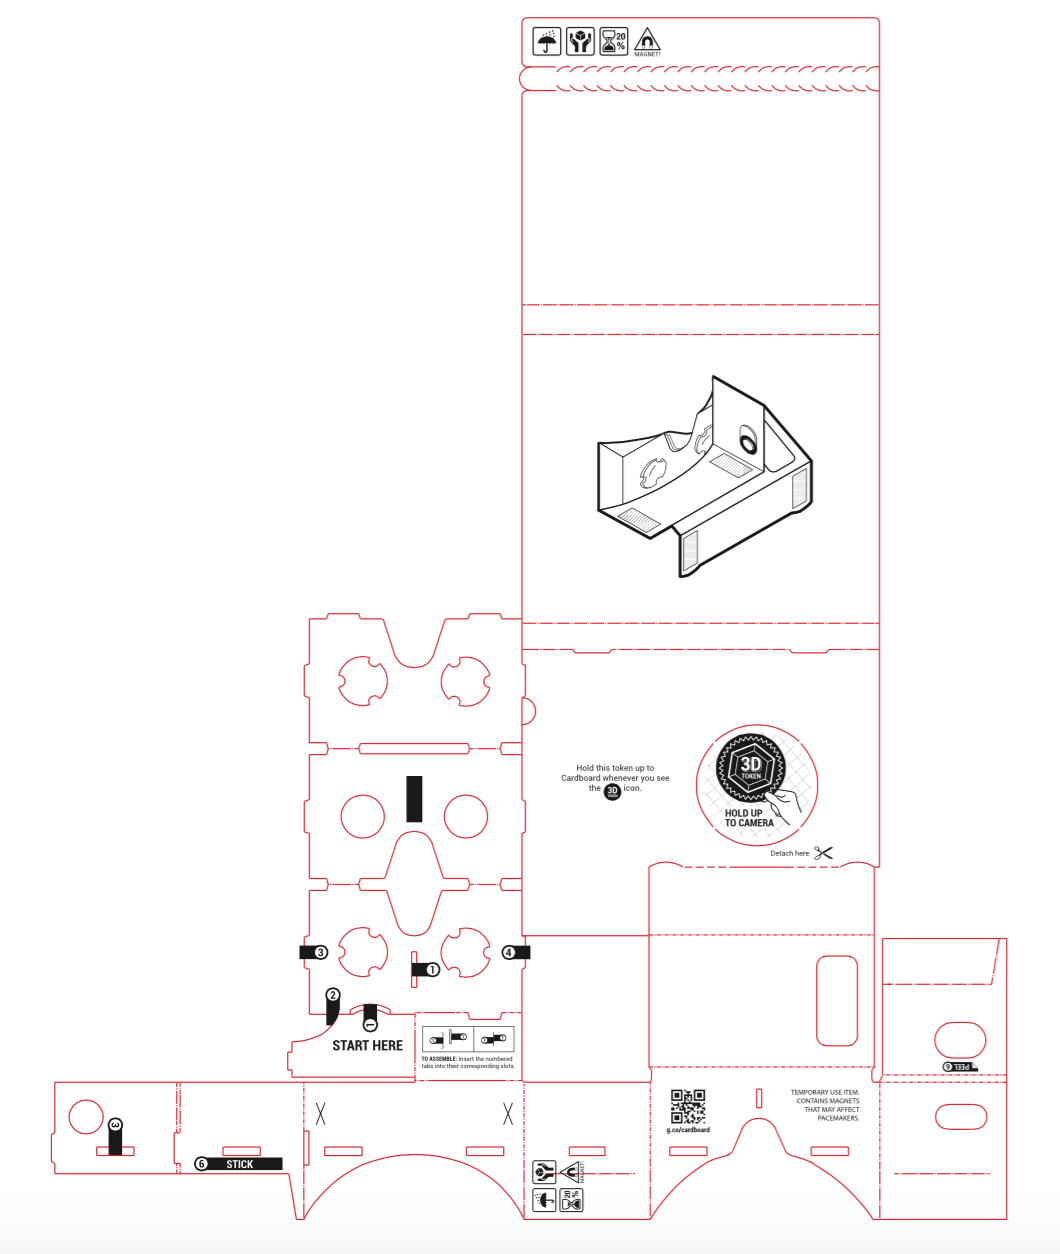
\includegraphics[width=100mm,scale=0.8]{Cardboard} \\ \\
%

\newpage\item\textbf{Lens}\\
Google Cardboard uses 45mm focal distance, asymmetric biconvex lenses. This type of lenses works best to prevent distortion around the edges. \\ 
\begin{enumerate}
\item Material needs to be optical PMMA or equivalent
\item All gates need to be trimmed flush
\item All contaminants need to be removed from surfaces 6. Lens needs to be RoHS and REACH compliant
\end{enumerate} 
\begin{center} 
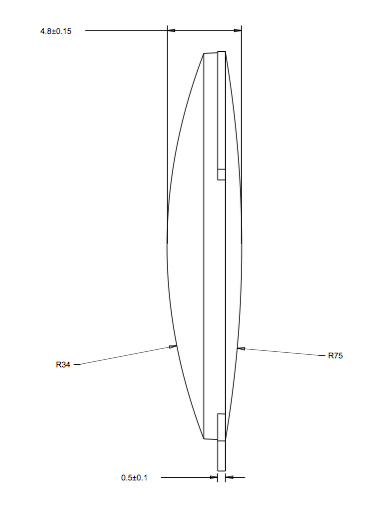
\includegraphics[width=50mm,scale=0.8]{lens1}\\
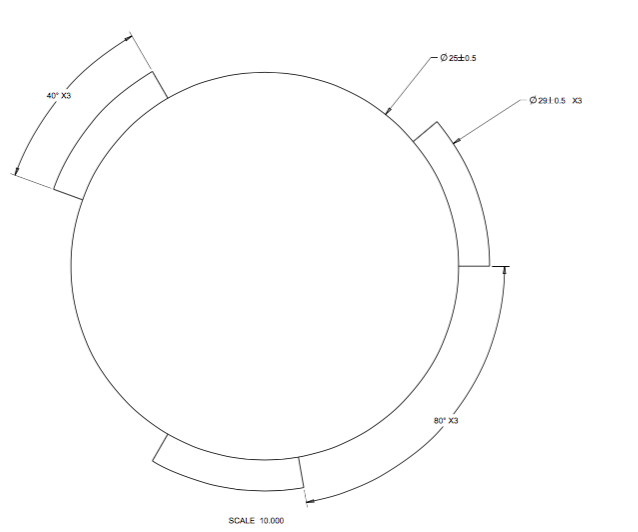
\includegraphics[width=50mm,scale=0.8]{lens2}\\
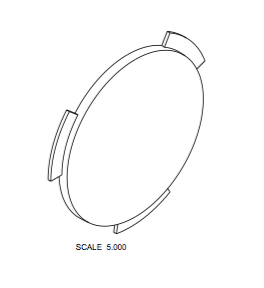
\includegraphics[width=50mm,scale=0.8]{lens3}\\
\end{center}
%
\newpage\item\textbf{Magnetic Pull}\\
If your viewer is using a magnet based input, use a neodymium ring magnet (at least NH35 grade) as an outside trigger. Google Cardboard ring magnet��s dimensions are 0.740�� x 0.105��.\\
\begin{center}
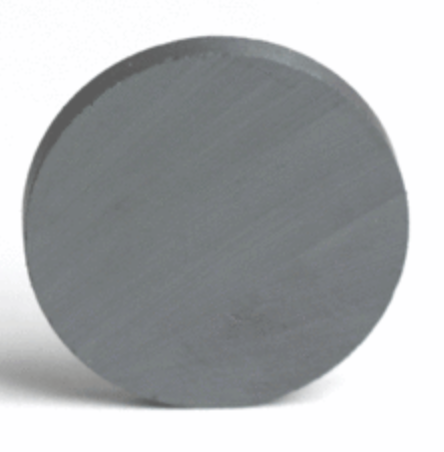
\includegraphics[width=50mm,scale=0.8]{magnet}\\
\end{center}
\item\textbf{Inputs}\\
\begin{enumerate}
\item Use a ceramic disk magnet with at least C8 grade for Cardboard inside. Ceramic magnet��s dimensions are 0.701�� x 0.197��. Make sure to glue the ceramic \item disk magnet in place, otherwise the whole magnet pair could come off easily and become a swallowing risk.
\item You can also use different types of inputs, from a simple smartphone screen touch, to Bluetooth-based buttons, various types of conductive and capacitive inputs, and so on.
\item Make sure that your viewer contains exactly one input. If your viewer uses the screen touch, ensure that there is at most one dedicated area for touching the screen.
\end{enumerate}

\item\textbf{Miscellaneous Google Cardboard parts (Velcro, stickers, rubber band, print)}
\begin{enumerate}
\item Google Cardboard uses two strips of regular-strength, adhesive-backed velcro. Approximate size is: 0.75�� x 1.25�� (20mm x 30mm). Make sure that the adhesive is sufficiently strong to not loosen from the cardboard top over time, as the strips will be getting a lot of use.
\item Similarly, make sure to use a strong adhesive sticker on the magnet side. This is what holds the whole assembly together, and it tends to loosen over time.
\item Use the rubber band to prevent the phone from sliding out. It is enough for the rubber band to be wrapped around the bottom of the viewer and touch the bottom of the phone it does not need to be wrapped around the box.
\end{enumerate}

\end{itemize}

\subsection{Requirement for Application Logo}
\begin{enumerate}
\item We designed our application logo, using Adobe Photoshop CS6 and Adobe Illustrator CS6.
\item Display it on the Smartphone.
\end{enumerate}

\subsection{Requirement for Loading page}
\begin{enumerate}
\item Show our application name
\item Show our team name
\end{enumerate}

\subsection{Requirement for Main page}
\begin{enumerate}
\item It would have five items
\item Panorama
\item 3D Cube
\item Volume
\item Preferences
\item Exit
\end{enumerate}

\subsection{Requirement for Panorama}
\begin{enumerate}
\item Click the Panorama Icon among the main page
\item Show the photographs of tourist attraction on the wall
\item To use gyroscope, users will  find the photograph which they want to go
\item Users will choose the photograph by pulling down the Magnetic pulling
\item Users are able to trip the attraction zone
\item If the tour is over, users could exit by back button
\end{enumerate}

\subsection{Requirement for Cine}
\begin{enumerate}
\item Click the Cine Icon among the main page
\item Show the movie poster on the notice board
\item To use gyroscope and Magnetic button, users will find the movie which they want to see and choose the movie
\item Users could be able to watch the movie to have experience the ambience of a movie theater
\item If the movie is over, users could exit by back button
\end{enumerate}

%Subsection 2
\subsection{Development Environment}

%subsubsection 2

\subsubsection{Choice of software development platform}
\begin{enumerate}
\item Our development platform is on OS X Yosemite. Our main reason for choosing the OSX is because it is built on top of UNIX, hence, the terminal is always ready waiting. Every Apple provides a variety of open source programming tools and frameworks built in such as: PHP, Apace, and Ruby on Rails. Our second reason is because of Quartz. Quartz is the OpenGL powered windowing system used by OSX. Quartz utilizes the graphics card exclusively, which means no processor cycles are taxed. This allows for a variety of useful features such as Expose, which dynamically resizes every window on the screen giving you a bird��s eye view of your entire workspace. When developing our application, it would sometime require us to open multiple windows.

\item Our main programming language is Java. Java is a very popular programming language developed by Sun Microsystems and owned by Oracle. Our main choice of Java is because it incorporates many of the powerful features with many powerful libraries and these libraries exist to help us build applications. Android relies heavily on the fundamentals of Java, and our developing tool (the Android Studio) includes Android SDK, which has many Java libraries. Therefore, it is easier for us to code and as well easier to understand. Another reason for choosing Java is because it is an object oriented language. Object oriented programming (in short OOP) is a programming style or technique that relies upon the definition of data structures called objects. To put it simpler, OOP is very much like a custom data type.

\item The total estimation cost of our built is 705,000 WON. First of all, we would need an android smartphone to test our application. We chose the Samsung Galaxy S6 because not only is it an Android Phone, but the specification of the smartphone would help us run our application much faster. Second of all, we would need the Google Cardboard sold by Google. Without this product our application would be useless.

\item Environment for testing and running code:
\begin{itemize}
\item 2.7GHz dual-core Intel Core i5 processor (Turbo Boost up to 3.1GHz) with 3MB shared L3 cache.
\item Android Studio Version 1.1.0
\item Samsung Galaxy S6 \\
Android OS, v5.0.2 (Lollipop)\\
Chipset Exynos 7420 \\
CPU Quad-core 1.5 GHz \\
Cortex-A53 and Quad-core 2.1 GHz 
\end{itemize}
\end{enumerate}

\newpage\subsubsection{Software in Use}
\begin{enumerate}
\item The Google Cardboard is originally built by Google. It was invented by David Coz and Damien Henry, whom are Google engineers at the Google Cultural Institute in Paris. It was recently introduced at the 2014 Google I/O developers conference. 

\item GitHub is a web-based Git repository hosting service, which offers all of the distributed revision control and source code management (SCM) functionality of Git as well as adding its own features. Unlike Git, which is strictly a command-line tool, GitHub provides a web-based graphical interface and desktop as well as mobile integration. It also provides access control and several collaboration features such as wikis, task management, and bug tracking and feature requests for every project.\\ \\
GitHub:\\
\begin{center}
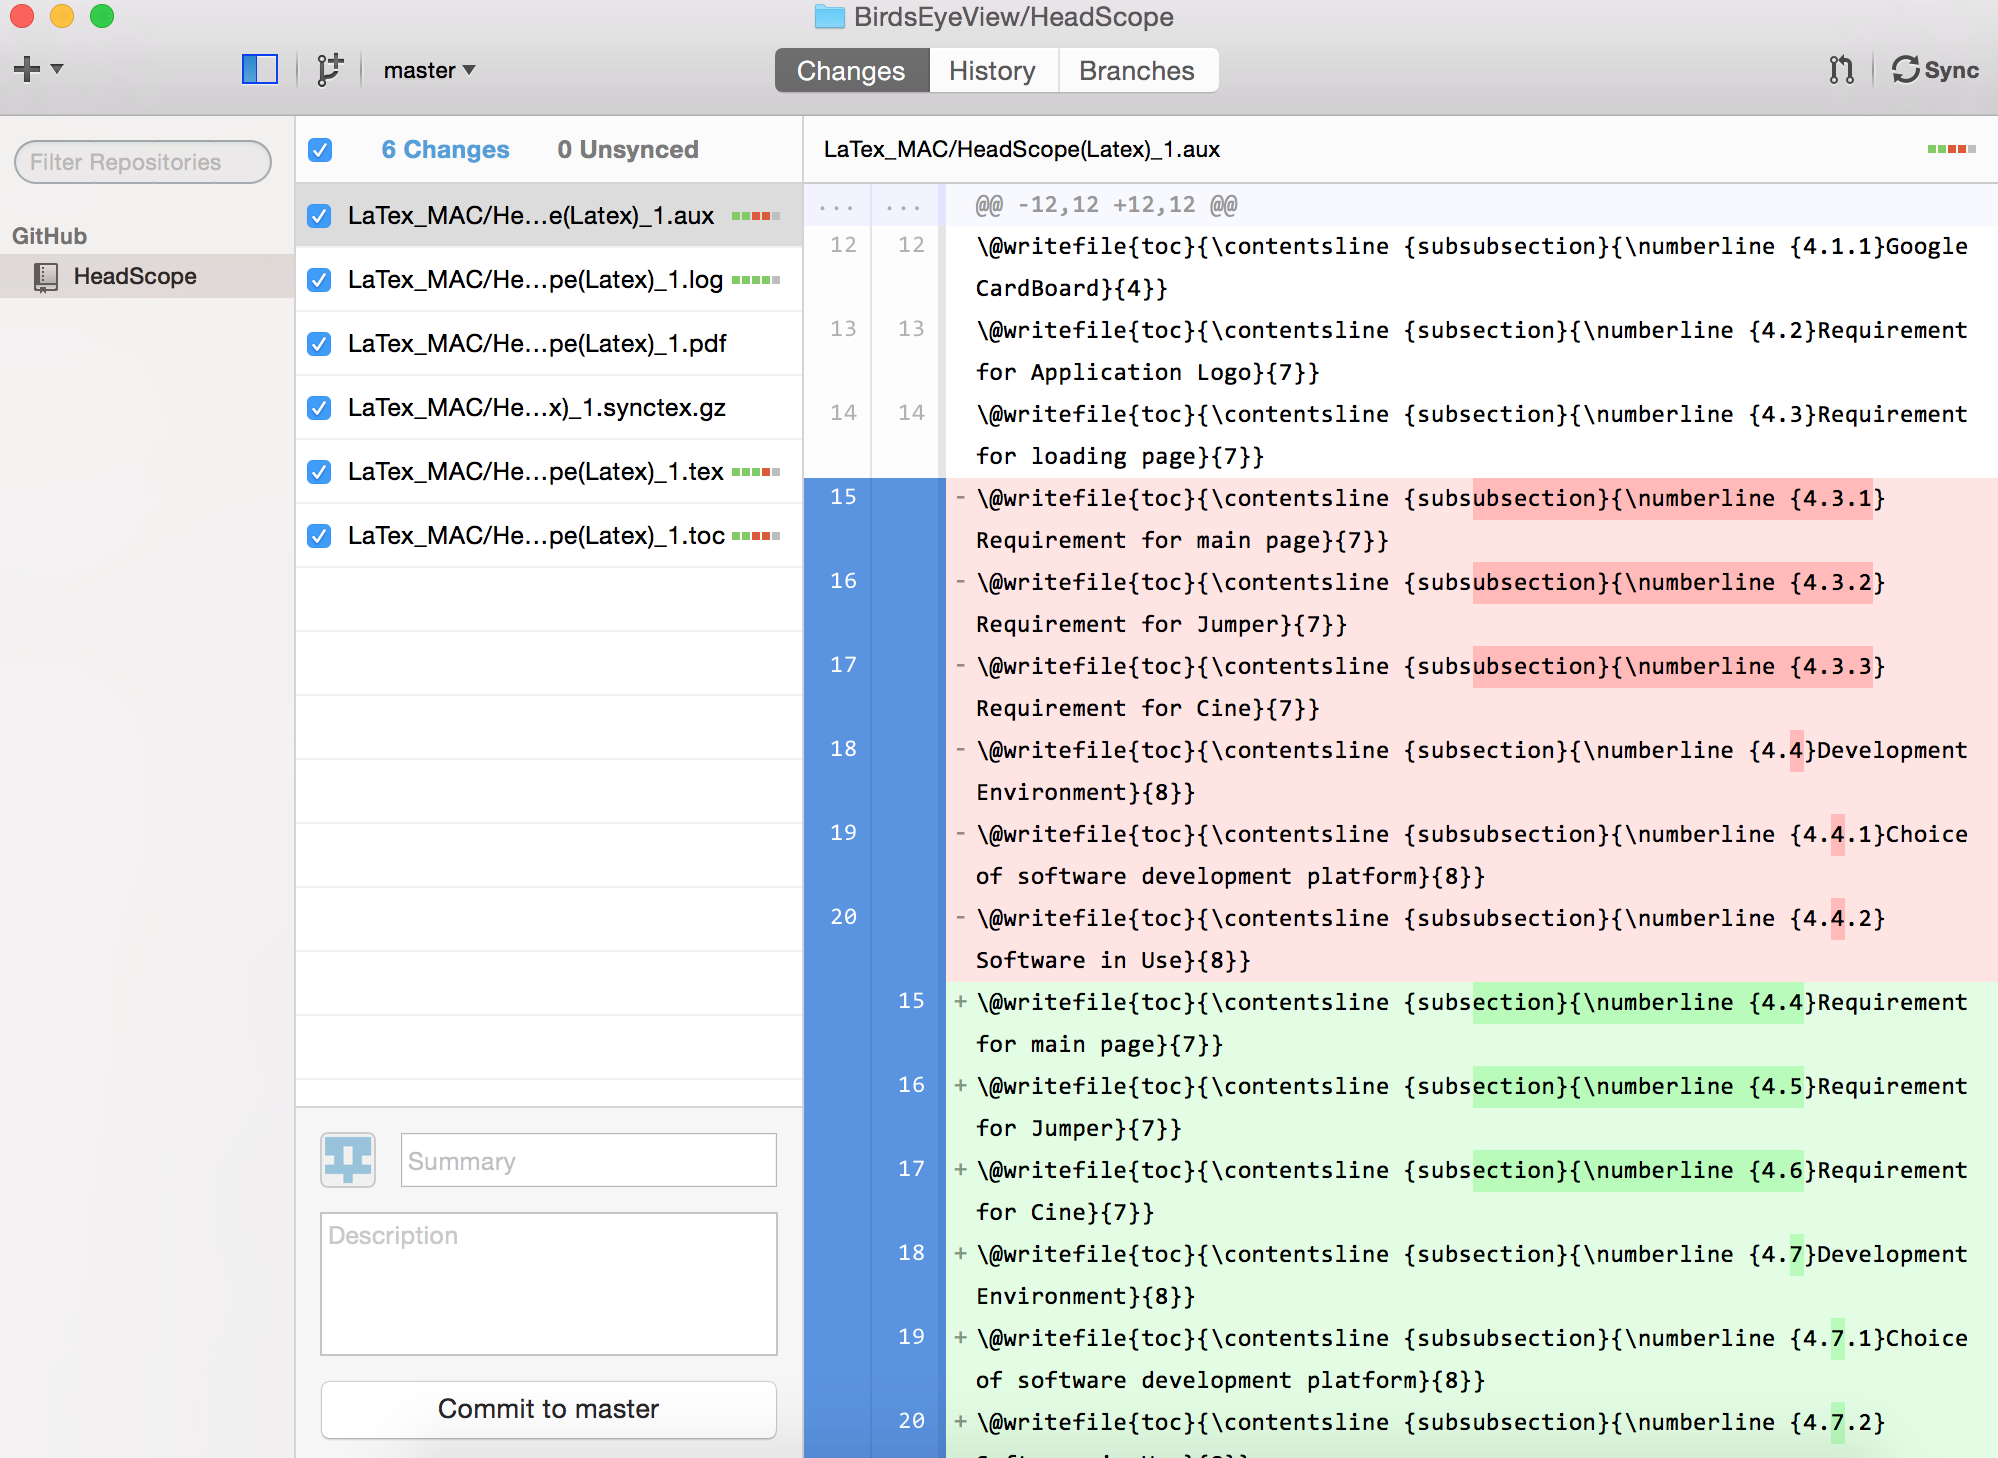
\includegraphics[width=140mm,scale=2]{Github}
\end{center}
\end{enumerate}

%subsection 3

\newpage \section{Specification}

%subsubsection 3

\subsection{Specification of App Icon}
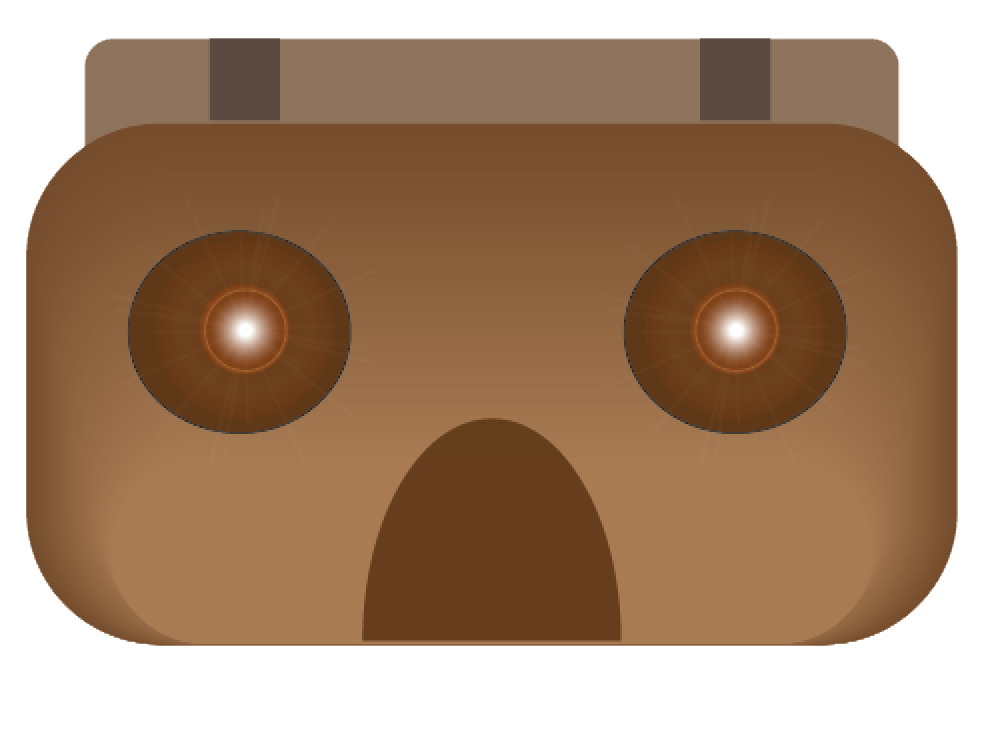
\includegraphics[width=50mm,scale=0.5]{HeadScope_APP}

%subsubsection 4
\subsection{Specification of Loading App Page}

\subsection{Specification of Main App Page}

\includegraphics{Main}
\begin{enumerate}
\item The Main App Page would have five applications:\\ \\
 Panorama\\
 3D Cube\\
 Volume\\
 Preferences\\
 Exit\\
\item Due to the gyroscope sensor built in the smartphone, we are able to select different apps inside the Main App Page by turning your head. We built a fixed cursor that will guide the users to what they are selecting. To select the desired app, users will simply pull down the magnetic pull.
\end{enumerate}

%subsubsection 5
\subsection{Specification of Panorama}
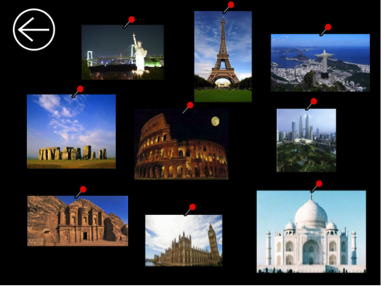
\includegraphics{Jumper}

\begin{enumerate}
\item The Panorama application will allow users to view an image in a 360 degree angle. This will give them a full view from the side to the back of an image by turning their head around. Panorama can give the users the experience to actually feel like their in that place. 
\item By using gyroscope, users will find the attraction place which they want to go and will choose the photograph.\\
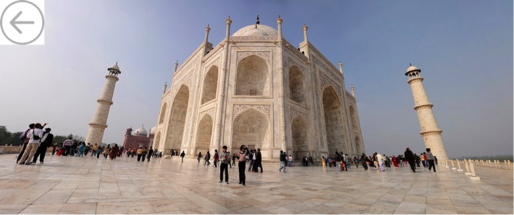
\includegraphics{View}
\item Since the image needs to be 360 degrees there are a limited number of images that we will be implementing. In addition, users are unable to upload their own image. However, our team will continue to update pictures from the famous attraction places such as: Namsan, Eiffel Tower, and even Egypt's Pyramids.
\end{enumerate}

%subsubsection 6
\subsection{Specification of 3D Cube}
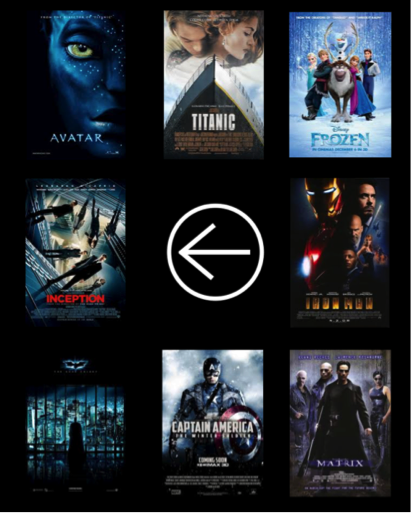
\includegraphics{Cine}

\begin{enumerate}
\item Upon clicking the 3D Cube App icon, users will search for the moving 3D Cube object. 
\item After the user find the 3D Cube, the users will lower the magnetic button that is installed in the Google Cardboard.
\item This will change the 3D Cube's color.
\item There is a point system within the app that counts the number of times the user find the 3D Cube object.
\end{enumerate}

%subsubsection 7
\subsection{Specification of Volume}

%includegraphics{} <-- image of the Volume icon

\begin{enumerate}
\item The Volume icon will adjust the amplification of the HeadScope application. 
\item Users are able to adjust the volume by turning their head towards the left for a lower sound and to right for a louder sound.
\end{enumerate}

%subsubsection 8
\subsection{Specification of Preferences}

%includegraphics{} <-- image of the Preference icon

\begin{enumerate}
\item The Preferences App Icon will display the settings based on the HeadScope App.
\item The first setting have a checkbox for smartphones that do not work with the magnetic pull. For those users whom smartphones do not support the Google Cardboards magnetic pull, there is an alternative. Users are able to select apps by holding the cursor shown in the smartphone steadily. Once the users hold the smartphone steadily there will be circle cursor that will fill when not moved. As soon as the circle is filled, the smartphone will select that app.
\item The second setting will contain a checkbox that makes the VR experience more seamless. This can create a smooth transition between apps without exiting the application.
\item The third setting is a function that allows the list of apps to be separated by commas, that the launcher will display.
\item The fourth setting has the same function of the third, but in a blacklist.
\item The fifth setting is the adjustment for the Interpupillary Distance. This setting is the distance between your pupils. 0 is set for pupils that are very
close and 100 for pupils that are far apart.
\item The sixth setting is a checkbox for users to disable vibration when selecting an app. When enabled, the phone will initiate a vibration upon selecting a desired application.
\item The seventh setting is a checkbox that will disable the volume buttons in the smartphone. Users will sometime experience situations where they accidentally press their smartphones volume button. For this case, we implemented an override method to disable the volume button when the HeadScope application is running.
\item The eight setting is premium checkbox that when clicked it will give direct users to our teams homepage. This is made just for users to donate to our project.
\item The ninth setting is a checkbox that allows users to modify the Main App Pages background. If not checked the Main App Page will have a default background which is the color of black.
\item The last setting is a checkbox that allows the voice recognition command. To launch the apps in the Main App Page users can also use the smartphones integrated voice command. This is an alternative choice for selecting apps instead of the magnetic pull.
 
 
\end{enumerate}

%Section 5
\section{Architecture Design and Implementation}
\subsection*{Overall Architecture}
\subsection*{Directory Organization}
\subsection*{Software Module for Launcher}

Software modules used in the "Home Launcher" is describe in form of different activities. Multiple activities have been used here to be handled by different functional requirements:
\lstset{
  language=Java,
  showstringspaces=false,
  columns=flexible,
  basicstyle={\small\ttfamily},
  numbers=none,
  numberstyle=\tiny\color{gray},
  keywordstyle=\color{blue},
  commentstyle=\color{dkgreen},
  stringstyle=\color{mauve},
  breaklines=true,
  breakatwhitespace=true,
  tabsize=3,
  escapeinside={<@}{@>}
}
\begin{lstlisting}
1.) private void onCreate(Bundle savedInstanceState)
-<@\textcolor{dkgreen}  {Function:}@> Called when the activity is starting. Calls method init()

2.) private void print(String request)
-<@\textcolor{dkgreen}  {Function:}@>prints out String request

3.) private void updateTweens()
-<@\textcolor{dkgreen}  {Function:}@>calculate accelData by adding tweenStep into original accelData

4.) private void prepareToLaunch()
-<@\textcolor{dkgreen}  {Function:}@>convert apps status to ready for launch by adjusting boolean startingApp to true

5.) private void launchApp()
-<@\textcolor{dkgreen}  {Function:}@>adjust AudioManager or call method launch()

6.) private void makeImmersive()
-<@\textcolor{dkgreen}  {Function:}@>compare android version (target SDK_INT >= KITKAT) if true set system ui visibility

7.) public boolean isMyAppLauncherDefault()
-<@\textcolor{dkgreen}  {Function:}@> add activity as a intent. add extra package to array list as an item
packageName.equals(activity.getPackageName())

8.) public boolean onKeyDown(int keyCode, KeyEvent event)
-<@\textcolor{dkgreen}  {Function:}@> compare keyCode to KeyEvent��s variables (back key, volume up/down key). return boolean.

9.) public boolean onCreateOptionsMenu(Menu menu)
-<@\textcolor{dkgreen}  {Function:}@> Inflate the menu. Add items to the action bar if it is present

10.) public boolean onOptionsItemSelected(MenuItem item)
-<@\textcolor{dkgreen}  {Function:}@>compare MenuItem item��s id to boolean which is calculated by R.id.action_settings or parent�� onOptionsItemSelected(Item)
	
11.) protected void onResume()
-<@\textcolor{dkgreen}  {Function:}@> for activity to start interacting with the user.
calls private SensorManager mSensorManager��s method registerListner that return true if the sensor is supported and successfully enabled.

12.) protected void onPause()
-<@\textcolor{dkgreen}  {Function:}@>called as part of the activity lifecycle when an activity is going into the background, but has not (yet) been killed.
calls private SensorManager mSensorManager��s method unregisterListner that unregisters a listener for all sensors

13.) public void onSensorChanged(SensorEvent sensorEvent)
-<@\textcolor{dkgreen}  {Function:}@> Calls when sensor values have changed

14.) public void onAccuracyChanged(Sensor sensor, int i)
-<@\textcolor{dkgreen}  {Function:}@> Called when the accuracy of the registered sensor has changed.

<@\textcolor{red}{public class MyView extends View\\ \\

Variables}@>

private Paint paint = new Paint();
private int width = 0;
private int height = 0;
private Rect cursorPosition = new Rect(width / 2 - 1, height / 2 - 1, width / 2 + 1, height / 2 + 1);
private int appStartAnimationPosition = 0;
private Rect freeAllocate = new Rect();
private int selectedApp = -1;
private long timeSelected = -1;
private final long selectionTime = 200;
long timeOfLastFrame = 0;
Display dis = ((WindowManager)getApplicationContext().getSystemService(Context.WINDOW_SERVICE)).getDefaultDisplay();
        Bitmap lEyeBit = Bitmap.createBitmap(dis.getWidth() / 2, dis.getHeight(), Bitmap.Config.ARGB_8888);
        Bitmap rEyeBit = Bitmap.createBitmap(dis.getWidth() / 2, dis.getHeight(), Bitmap.Config.ARGB_8888);
        Canvas lEye = new Canvas(lEyeBit);
        Canvas rEye = new Canvas(rEyeBit);

15.) constructor public MyView(Context context)
-<@\textcolor{dkgreen}  {Function:}@> sets variable to super(context), paint, width, volumePanelWidth, height, timeOfLastFrame. calls method gameloop()

16.) private void gameLoop()
-<@\textcolor{dkgreen}  {Function:}@> calls method move(), updateTweens, invalidate()
if width is 0, then reset width, volumePanelWidth, height, cursorPosition
if selectedApp is -1 calls for loop installedApps.size() times
reset rectangle freeAllocate, selected, timeSelected
if starting app
then calls method launchApp() or modify appStartAnimationPosition

17.) public void magnetPull()
-<@\textcolor{dkgreen}  {Function:}@>adjust volume or reset rotation

float headMatrix[] = new float[16];
float headFloats[] = new float[3];

18.) private void move()
-<@\textcolor{dkgreen}  {Function:}@> adjust volumePanelKnobPosition. set installedApps variable through for loop.

19.) float[] getEulerFromMat(float[] rotMatrix)
local variable : 
float x, y, z;
float _11, _12, _13, _14;
float _21, _22, _23, _24;
float _31, _32, _33, _34;
float _41, _42, _43, _44;

-<@\textcolor{dkgreen}  {Function:}@> set array rotMatrix values to float _11~_44. calculate x, y, z and return float array[x, y, z]

20.) public float[][] matrixMultiply(float[][] A, float[][] B)
local variable : 
int aRows = A.length;
int aColumns = A[0].length;
int bRows = B.length;
int bColumns = B[0].length;

-<@\textcolor{dkgreen}  {Function:}@> calculate variables. set multiple array C value. return C

21.) protected void onDraw(Canvas canvas)

-<@\textcolor{dkgreen}  {Function:}@> Draw left, right eyes by using canvas class. Render eyes to screen. Draw screen divider
Call method gameLoop()

22.) public boolean onTouchEvent(MotionEvent motionEvent)
-<@\textcolor{dkgreen}  {Function:}@>Call method magnetPull(). return boolean false


\end{lstlisting}

\newpage \subsection*{Software Module of Panorama}

MainActivity
\begin{itemize}
\item Act as main class
\item Attach current view to cardboard view class
\item Attach current view renderer to renderer class
\end{itemize}
MyRenderer
\begin{itemize}
\item Input drawable resource to current scene by using initScene()
\end{itemize}
Rajawali 
\begin{itemize}
\item 3D engine for Android based on OpenGL ES 2.0/3.0.
\end{itemize}
RajawaliCardboardView
\begin{itemize}
\item View class which attach current context
\end{itemize}
\begin{itemize}
\item IRajawaliSurface is an Interface which all rendering surfaces must implement so that RajawaliRenderer may send the few control signals it needs.
\end{itemize}
RajawaliCardboardRenderer
\begin{itemize}
\item Apply the eye transformation to the camera
\item Call openGL10 as a object, define openGL methods
\item Called as the user performs touch-screen interaction with the window that is currently showing this wallpaper
\end{itemize}
\end{document}






